\documentclass[12 pt]{article}
\usepackage{fancyhdr}
\usepackage[margin = 1 in]{geometry}
\usepackage{amsmath}
\usepackage{enumerate}
% \usepackage{indentfirst}
\pagestyle{fancy}
\usepackage{graphicx}
\usepackage[version=3]{mhchem}
\fancyhf{}
\usepackage{sectsty}	
\lhead{Andrew Wang}
\chead{CS/CNS/EE 155 Machine Learning \& Data Mining}
\rhead{Yue}
\sectionfont{\fontsize{15}{18}\selectfont}
\usepackage{graphicx}
\usepackage{array}
\newcolumntype{P}[1]{>{\centering\arraybackslash}p{#1}}
\newcolumntype{M}[1]{>{\centering\arraybackslash}m{#1}}
\usepackage[font=small,labelfont=bf]{caption}
\usepackage{float}
\usepackage{float}
\usepackage{subfig}
\usepackage{microtype}
\usepackage{ amssymb }
\usepackage{amsmath}
\usepackage{commath}
\begin{document}
	\begin{center}
		\section*{Homework [INSERT]}
	\end{center}
	
	
	\subsection*{1 [INSERT]}	
	\noindent\textbf{Question A:}  \\
	
	\noindent\textbf{Question B:}  \\
	
	\noindent\textbf{Question C:}  \\
	
	\noindent\textbf{Question D:}  \\
	
	\noindent\textbf{Question E:}  \\
	
	\noindent\textbf{Question F:}  \\
	
	\noindent\textbf{Question G:} \\
	
	\noindent\textbf{Question H:} 
 
	
	\subsection*{2 [INSERT]}
	\noindent\textbf{Question A:} \\
	
	\noindent\textbf{Question B:} \\

	%\begin{figure}[h]
	%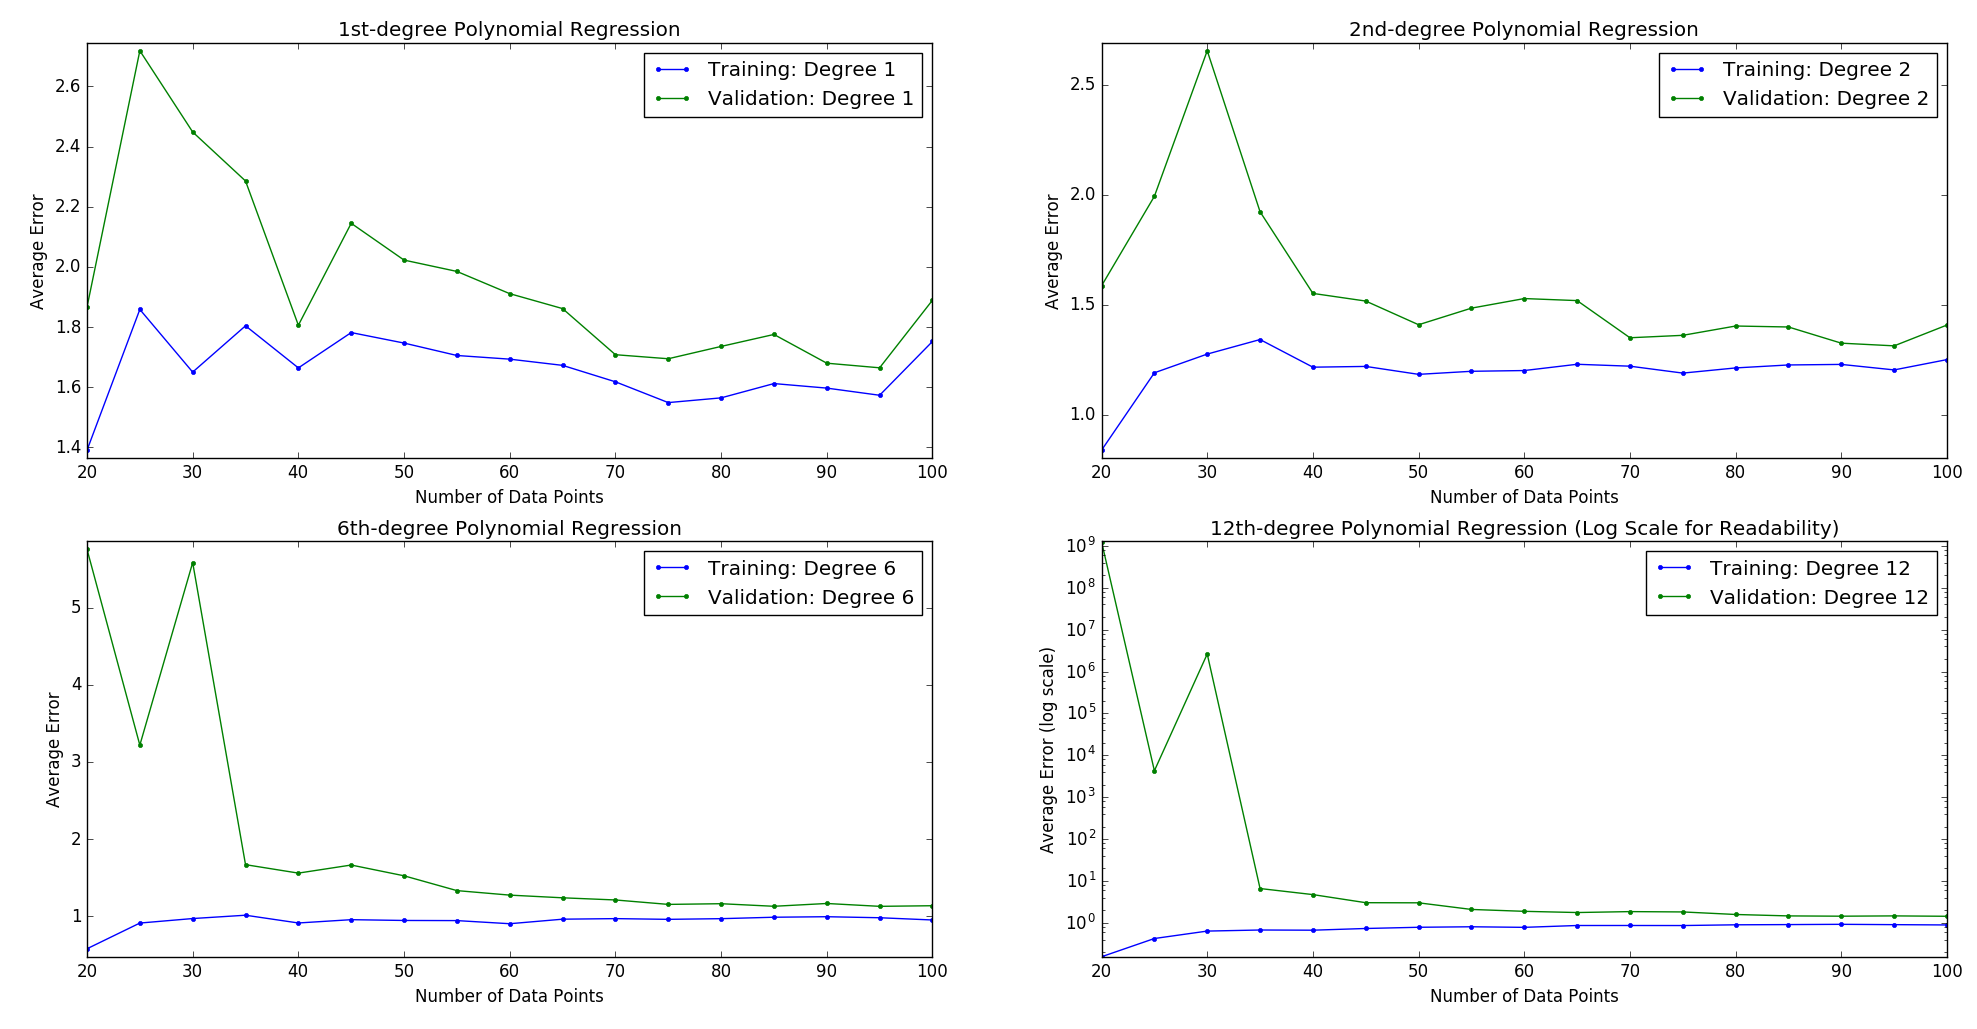
\includegraphics[width=17cm]{LearningCurves}
	%\end{figure}	
	
	\noindent\textbf{Question C:}  \\
	
	\noindent\textbf{Question D:} \\
	
	\noindent\textbf{Question E:} \\
	
	\noindent\textbf{Question F:} \\
	
	\noindent\textbf{Question G:} 
	
	\subsection*{3 [INSERT]}
	\noindent\textbf{Question A:} \\

	
	\noindent\textbf{Question B:} \\

	
	\noindent\textbf{Question C:} 
	
	\subsection*{4 [INSERT]}
	\noindent\textbf{Question A:} \\
	
	\noindent\textbf{Question B:} \\

	
	\noindent\textbf{Question C: } \\
	
	\noindent\textbf{Question D:} \\


	\noindent\textbf{Question E:} \\
	
	\noindent\textbf{Question F:} \\
	
	\noindent\textbf{Question G:} 
	
\end{document}